% Main file for the MAT386 VIX group report.
% Compile from the report/ folder:   latexmk -pdf main.tex
% Each member edits only their own file in sections/; the shared preamble lives here.

\documentclass[11pt,a4paper]{article}

\usepackage[margin=2.5cm]{geometry}
\usepackage[T1]{fontenc}
\usepackage[utf8]{inputenc}
\usepackage{amssymb, amsmath, amsbsy, amsthm, amsfonts}
\usepackage{enumerate}
\usepackage{array}
\usepackage{graphicx}
\usepackage{booktabs}
\usepackage{float}
\usepackage{caption}
\usepackage{xcolor}
\usepackage[colorlinks=true,linkcolor=blue!50!black,citecolor=blue!50!black,urlcolor=blue!50!black]{hyperref}

% headers
\usepackage{fancyhdr}
\setlength{\headheight}{15pt}
\usepackage{lastpage}
\pagestyle{fancy}
\fancyhf{}
\lhead{MAT386H5 -- Fall 2026}
\rhead{VIX and VIX Derivatives}
\cfoot{\thepage\ of \pageref{LastPage}}

% shared commands
\newcommand{\verify}[1][]{\textcolor{red}{\textsuperscript{[verify#1]}}}  % flag claims that still need a source
\newcommand{\figplaceholder}[2]{\fbox{\parbox[c][#1][c]{0.9\linewidth}{\centering\textit{#2}}}}
\newcommand{\todo}[1]{\textcolor{red}{\textit{[To do: #1]}}}
\newcommand{\E}{\mathbb{E}}
\newcommand{\EQ}{\mathbb{E}^{\mathbb{Q}}}
\newcommand{\VIX}{\mathrm{VIX}}
\newcommand{\Kvar}{K_{\mathrm{var}}}

\title{VIX and VIX Derivatives}
\author{MAT386 Group Project --- Nikita, Tony, Josh, Daniel}
\date{November 2026}

\begin{document}
\maketitle

\begin{abstract}
\noindent
This report studies the Cboe Volatility Index (VIX) and the derivatives written on it. We introduce the VIX as the market's ``fear gauge'' and the products that trade volatility directly, specify the VIX methodology and contracts, derive VIX$^2$ as the fair strike of a 30-day variance swap, and implement the Cboe formula on live S\&P~500 option quotes, matching the official index to within 0.05 points. Under a Heston model started at the spot VIX, we price VIX futures and calls by Monte Carlo and show that the convexity adjustment, the gap between the square root of forward variance and the VIX future, grows from 0.6 points at one month to 2.3 points at six months; the one-factor model cannot reproduce the shape of the market futures curve. Finally, a 2015--2026 backtest of a rolling, variance-minimising VIX-futures hedge on a \$1M S\&P~500 portfolio cuts the loss in the COVID crash from 33\% to under 2\%, but the cost of rolling futures in contango lowers the annual return from 13.5\% to 8--9\%.
\end{abstract}

\tableofcontents
\newpage

%=====================================================================
\section{Discussion}
%=====================================================================
% Discussion (Josh). Moved from paper/vix_discussion.tex; headings demoted one level, preamble moved to main.tex.

\subsection{The VIX as the Market's ``Fear Gauge''}
\subsubsection{What the VIX measures}

The VIX is an index published by Cboe that measures the stock market's \emph{expected} volatility of the S\&P~500 over the next 30 calendar days. It is quoted in annualized percentage points. The VIX is \emph{forward-looking}: it is computed from the market prices of S\&P~500 index options, and is therefore a form of \emph{implied} volatility \cite{cboewp}. This is in contrast to historical (realized) volatility, which looks backward at past returns. 

Using the annualized convention, a VIX of $20$ corresponds to an expected one-standard-deviation move of the S\&P~500 over one month of about
\begin{equation}
  \frac{20\%}{\sqrt{12}} \approx 5.8\%.
\end{equation}

For a single option expiration with time to maturity $T$, Cboe calculates the annualized forward variance $\sigma^2$ as
\begin{equation}
  \sigma^2 = \frac{2}{T}\sum_i \frac{\Delta K_i}{K_i^2}\,e^{RT}\,Q(K_i)\;-\;\frac{1}{T}\left(\frac{F}{K_0}-1\right)^{2},
  \label{eq:vix-term}
\end{equation}
where:
\begin{itemize}
  \item $T$ is the time to expiration in calendar years, computed to the minute as $T = M / 525{,}600$, where $M$ is the number of minutes until settlement.
  \item $R$ is the risk-free interest rate to expiration (continuously compounded from Treasury yields).
  \item $F$ is the option-implied forward index level, derived from at-the-money put-call parity as $F = K^* + e^{RT}(C(K^*) - P(K^*))$, where $K^*$ is the strike minimizing $|C(K) - P(K)|$.
  \item $K_0$ is the strike price equal to or immediately below $F$.
  \item $K_i$ is the strike price of the $i$-th selected option. Out-of-the-money puts are used for $K_i < K_0$ and out-of-the-money calls for $K_i > K_0$.
  \item $Q(K_i)$ is the mid-quote price of the option at strike $K_i$. At $K_0$, both the call and put options are included, and $Q(K_0) = \frac{1}{2}\big(Q_{\text{put}}(K_0) + Q_{\text{call}}(K_0)\big)$.
  \item $\Delta K_i = \frac{1}{2}(K_{i+1} - K_{i-1})$ is the strike interval (with $\Delta K_1 = K_2 - K_1$ and $\Delta K_N = K_N - K_{N-1}$ at the truncation boundaries).
\end{itemize}

Because listed options rarely expire in exactly 30 days, Cboe selects two expirations bracketing 30 days (a near-term expiration $T_1$ and a next-term expiration $T_2$, with $23 < \text{days} < 37$) and computes $\sigma_1^2$ and $\sigma_2^2$ using~\eqref{eq:vix-term}. The 30-day spot VIX is then obtained via constant-maturity linear variance interpolation:
\begin{equation}
  \VIX = 100 \times \sqrt{ \left\{ T_1 \sigma_1^2 \left( \frac{N_{T_2} - N_{30}}{N_{T_2} - N_{T_1}} \right) + T_2 \sigma_2^2 \left( \frac{N_{30} - N_{T_1}}{N_{T_2} - N_{T_1}} \right) \right\} \frac{N_{365}}{N_{30}} },
  \label{eq:vix-interp}
\end{equation}
where $N_{T_1}$ and $N_{T_2}$ are the minutes to settlement for the two expirations, $N_{30} = 43{,}200$ minutes (30 days), and $N_{365} = 525{,}600$ minutes (365 days). The theoretical derivation of~\eqref{eq:vix-term} from variance-swap replication is presented in the pricing section of this report.


\subsubsection{Why it is called the fear gauge}

Investors who fear a market decline buy protection, typically out-of-the-money put options. Higher demand raises option prices and thus implied volatility. Equity returns and the VIX are strongly negatively correlated: the VIX tends to rise sharply when the S\&P~500 falls, and to drift lower in calm, rising markets. This asymmetry explains why VIX products are attractive as portfolio hedges.

Typical levels are roughly 10--15 in calm markets, a long-run average near 19--20, and readings well above 40 in crises such as late 2008 and March 2020 \cite{whaley}.

\begin{figure}[H]
  \centering
  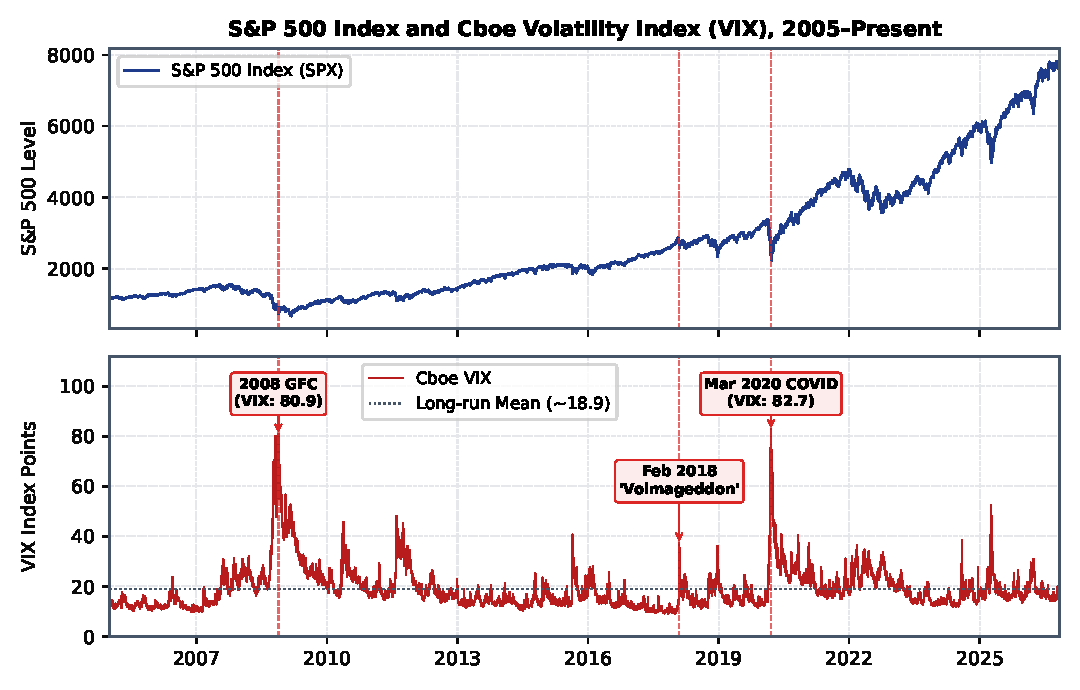
\includegraphics[width=0.9\linewidth]{figures/vix_vs_spx.pdf}
  \caption{S\&P~500 (top) and VIX (bottom), daily closes, January 2005 -- November 2026. Dotted lines mark 20 November 2008, 5 February 2018, and 16 March 2020; the dashed line is the average VIX over the period. Data: Yahoo Finance (\texttt{\textasciicircum GSPC}, \texttt{\textasciicircum VIX}).}
  \label{fig:vix-spx}
\end{figure}

\subsection{Trading Volatility Directly}
\subsubsection{Why volatility is hard to trade}

The VIX is a calculation, not a tradable asset: it cannot be bought, stored or delivered. Before volatility derivatives existed, investors could gain exposure to volatility only indirectly, for instance through delta-hedged option positions, which require continual rebalancing and carry other risks. Listed volatility products give a \emph{direct} and cheap way to take a view on volatility itself.

\subsubsection{The VIX product family}

Cboe introduced the VIX in 1993, adopted the current option-based methodology in 2003, launched VIX futures in 2004 and VIX options in 2006 \cite{cboewp}. Exchange-traded products linked to VIX futures followed from 2009 onward \cite{vxx}. Table~\ref{tab:products} summarizes the main instruments.

\begin{table}[H]
\centering
\small
\begin{tabular}{@{}p{3.4cm}p{3.6cm}p{3.6cm}p{4.2cm}@{}}
\toprule
\textbf{Product} & \textbf{Type} & \textbf{Underlying} & \textbf{Typical use}\\
\midrule
VIX Futures (\texttt{VX}) & Exchange-traded futures & Spot VIX at settlement & Portfolio hedging, directional speculation\\
\addlinespace
VIX Options & European cash-settled options & Spot VIX at settlement & Tail-risk hedging, asymmetric volatility bets\\
\addlinespace
Long VIX ETPs (\texttt{VXX}) & Exchange-traded note / fund & Rolling short-term VIX futures & Tactical short-term crash protection\\
\addlinespace
Inverse VIX ETPs (\texttt{SVXY}, \texttt{XIV}) & Inverse ETN / ETF & Rolling short VIX futures (daily reset) & Harvesting volatility risk premium\\
\addlinespace
Leveraged VIX ETPs (\texttt{UVXY}) & Leveraged ETN / ETF & Rolling leveraged VIX futures (daily reset) & Magnified short-term volatility exposure\\
\bottomrule
\end{tabular}
\caption{Overview of VIX-linked products.}
\label{tab:products}
\end{table}

\subsubsection{Why investors trade VIX products}

\begin{itemize}
  \item \textbf{Hedging.} Because the VIX rises when equities fall, a long volatility position can offset losses in an equity portfolio.
  \item \textbf{Speculation.} Investors can express views on the level of volatility or on changes in market stress.
  \item \textbf{Volatility risk premium.} Implied volatility tends on average to exceed subsequently realized volatility, so systematically selling volatility earns a premium, but with the risk of large losses in crashes.
\end{itemize}

\subsection{VIX Exchange-Traded Products}
\subsubsection{How VXX works}

The iPath S\&P~500 VIX Short-Term Futures ETN (ticker \texttt{VXX}) was launched by Barclays Bank PLC in January 2009. Upon the scheduled 10-year maturity of the original notes in January 2019, it was replaced by the Series~B notes (initially launched as \texttt{VXXB} in January 2018 and subsequently renamed \texttt{VXX}) \cite{vxx}. VXX tracks the S\&P~500 VIX Short-Term Futures Index, which targets a constant maturity of approximately 30 days by holding a rolling position in the first- and second-month VIX futures contracts. Two structural features are essential:

\begin{enumerate}
  \item VXX tracks \emph{futures}, not the spot VIX; the two can differ substantially.
  \item VXX is an exchange-traded \emph{note}: it is an unsecured debt obligation of the issuer, so holders also bear issuer credit risk \cite{vxx}.
\end{enumerate}

If $d_r$ business days remain before the first future expires and the current roll period contains $d_t$ business days, the index weights are
\begin{equation}
  w_1 = \frac{d_r}{d_t},\qquad w_2 = 1-w_1,
  \qquad
  F^{\text{(30d)}} \approx w_1F_1 + w_2F_2,
  \label{eq:weights}
\end{equation}
where $F_1,F_2$ are the first- and second-month VIX futures prices. Each day exposure shifts from $F_1$ towards $F_2$, so the product continually sells the nearer future and buys the next.

\subsubsection{Roll yield and the decay of long-volatility ETPs}

Under normal conditions the VIX futures curve is in \emph{contango}: later-dated futures trade above the spot VIX (see the term-structure discussion in the next section). A future converges to the spot VIX at expiry, so if spot VIX does not move, a long position in the future $F_0$ earns
\begin{equation}
  \text{P\&L} \approx S_T - F_0 = -(F_0 - S_0) < 0 .
  \label{eq:roll}
\end{equation}
Spread over the remaining life of the contract, the daily convergence loss is roughly $-(F_1-S)/d_r$ per unit. Because VXX must roll continually, this loss recurs, a phenomenon known as \emph{negative roll yield}. As a result VXX has lost the vast majority of its value since inception (its split-adjusted price has declined by over 99.9\% via repeated reverse splits), even though the VIX itself has no such trend. This is the central reason why VIX ETPs are poor long-term holdings and are intended as short-term instruments.

\begin{figure}[H]
  \centering
  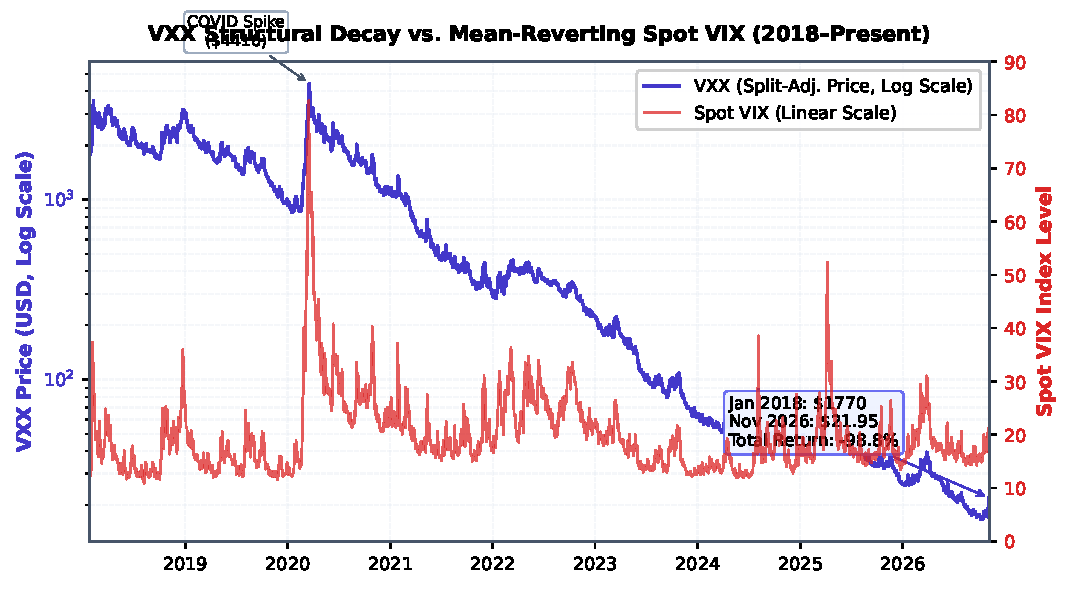
\includegraphics[width=0.9\linewidth]{figures/vxx_vs_vix.pdf}
  \caption{VXX decays over time despite a mean-reverting VIX. This persistent loss reflects negative roll yield caused by contango in the futures curve (split-adjusted price, log scale). Data: Yahoo Finance.}
  \label{fig:vxx}
\end{figure}

\subsubsection{Inverse and leveraged products}

Inverse products such as XIV and SVXY take the opposite side: they earn the roll yield in contango but lose when volatility spikes. Because leveraged and inverse products reset their exposure \emph{daily}, their return over several days is path-dependent. If the underlying futures return is $r$ over one day, a $-1\times$ inverse product's net asset value is multiplied by
\begin{equation}
  1 - r .
  \label{eq:inverse}
\end{equation}
A one-day futures rise of $r\geq 100\%$ would therefore wipe the product out entirely, and a rise of $r=90\%$ would leave only $10\%$ of its value.

There is also a mechanical feedback effect. To restore $-1\times$ exposure at the close after a spike, an inverse product must \emph{buy} VIX futures, which adds to the very rally that caused the losses \cite{augustin}.

\subsection{Volmageddon (February 2018)}
\subsubsection{Background}

After a long period of low volatility, with the VIX near 9--12 in late 2017, short-volatility strategies had been extremely profitable and inverse VIX ETPs such as XIV and SVXY had grown large, holding about \$3.6~billion between them on 5 February 2018 \cite{bbgvol}. This set the stage for a violent reversal.

\subsubsection{Timeline}

\begin{table}[H]
\centering
\small
\begin{tabular}{@{}p{3.6cm}p{11cm}@{}}
\toprule
\textbf{Date} & \textbf{Event}\\
\midrule
Late Jan.--2 Feb.\ 2018 & Equity sell-off begins after a strong January rally\\
5 Feb.\ 2018 & S\&P~500 falls about 4\%; VIX roughly doubles in a day (+115.6\%), its largest one-day percentage rise on record\\
5 Feb.\ 2018, after close & XIV's indicative value falls by 96\% (from \$108.37 to \$4.22)\\
6--21 Feb.\ 2018 & Issuer (Credit Suisse) accelerates (6 Feb.) and terminates XIV (final cash settlement on 21 Feb.) \cite{csxiv}\\
\bottomrule
\end{tabular}
\caption{Key events of the Volmageddon episode.}
\label{tab:timeline}
\end{table}

\subsubsection{Why the products broke}

Three mechanisms combined:
\begin{enumerate}
  \item \textbf{Short exposure to a bounded-below, unbounded-above variable.} By~\eqref{eq:inverse}, a large rise in VIX futures implies a loss approaching 100\% for an inverse product in a single day.
  \item \textbf{Daily rebalancing feedback.} Buying futures near the close to restore exposure amplified the spike in futures prices \cite{augustin}.
  \item \textbf{Termination provisions.} The XIV notes allowed the issuer to accelerate the product if the indicative value fell by 80\% or more in one day (specifically, if intraday indicative value was $\le 20\%$ of the previous day's close) \cite{csxiv}.
\end{enumerate}

\begin{figure}[H]
  \centering
  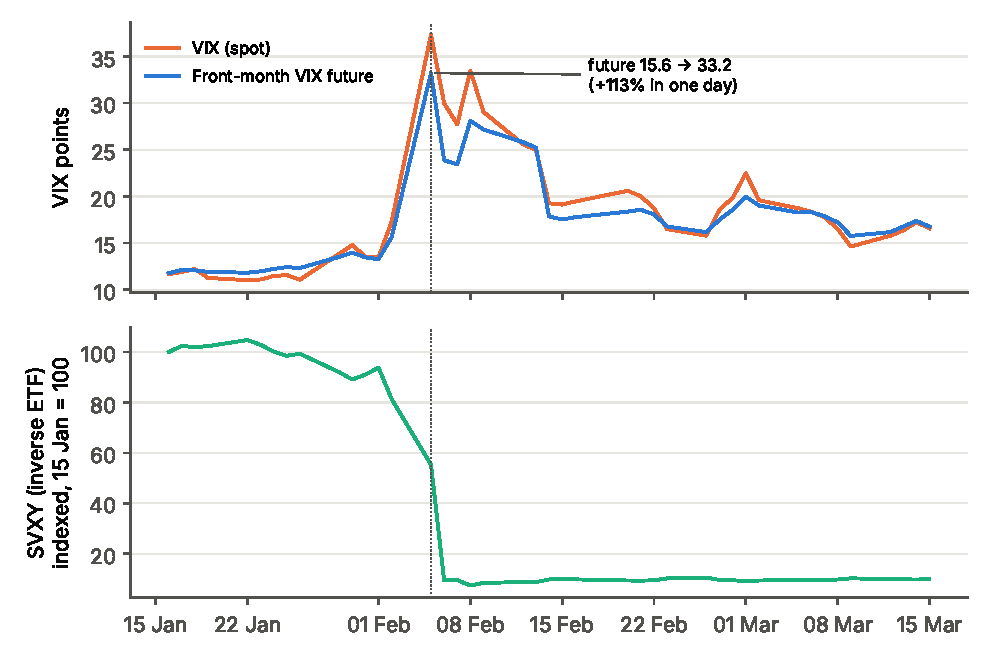
\includegraphics[width=0.9\linewidth]{figures/volmageddon.pdf}
  \caption{Top: VIX and the front-month VIX future, 15 January -- 15 March 2018; on 5 February the front-month future rose from 15.6 to 33.2. Bottom: the inverse VIX ETF SVXY, indexed to 100 on 15 January. Data: Yahoo Finance, Cboe Futures Exchange settlement prices.}
  \label{fig:volmageddon}
\end{figure}

\subsubsection{Aftermath and lessons}

After the event, regulators and exchanges paid closer attention to leveraged and inverse ETPs, and surviving products were redesigned (for example, SVXY reduced its target exposure from $-1.0\times$ to $-0.5\times$) \cite{proshares}. The main lessons are: (i) selling volatility earns a premium but carries severe crash risk; (ii) daily-reset products are path-dependent and unsuitable for buy-and-hold; and (iii) the structure of a product, including issuer risk and termination clauses, matters as much as its underlying exposure.

\subsection{Link to the Rest of the Report}
The next sections specify the VIX methodology and futures contract in detail, including the term structure (contango versus backwardation); derive $\VIX^2$ as the fair strike of a 30-day variance swap and quantify the convexity adjustment; and implement the Cboe formula, a Heston simulation and a backtest of a VIX-futures hedge including roll yield.


%=====================================================================
\section{Product specification}
%=====================================================================
\todo{Cboe VIX methodology (30-day variance from a strip of S\&P~500 options, interpolated between two maturities); VIX futures (\$1{,}000 multiplier, cash settlement on the Special Opening Quotation); VIX options (\$100 multiplier, European, SOQ settlement); futures term structure (contango vs backwardation). The methodology formula currently sits in Section~1.1.1 and could move here.}

%=====================================================================
\section{Pricing and hedging}
%=====================================================================
% Pricing & hedging: VIX^2 as the fair strike of a variance swap (Nikita).

\subsection{VIX$^2$ as the fair strike of a variance swap}
\subsubsection{Setup}

We work under the risk-neutral measure $\mathbb{Q}$ with a constant interest rate $r$ and dividend yield $q$. The S\&P~500 index $S_t$ follows a diffusion whose volatility $\sigma_t$ may itself be random, so the result holds for the Heston model and any other stochastic-volatility model without jumps:
\begin{equation}
  \frac{dS_t}{S_t} = (r-q)\,dt + \sigma_t\,dW_t .
\end{equation}
The forward price for delivery at $T$ is $F_t = S_t e^{(r-q)(T-t)}$. It has no drift under $\mathbb{Q}$, and $F_T = S_T$:
\begin{equation}
  \frac{dF_t}{F_t} = \sigma_t\,dW_t .
  \label{eq:fwd}
\end{equation}
A variance swap with maturity $T$ pays, per unit of notional, the realised variance minus a strike $\Kvar$ agreed today. It costs nothing to enter, so the fair strike is the risk-neutral expectation of realised variance:
\begin{equation}
  \text{Payoff} = \frac{1}{T}\int_0^T \sigma_t^2\,dt - \Kvar,
  \qquad
  \Kvar = \EQ\!\left[\frac{1}{T}\int_0^T \sigma_t^2\,dt\right].
\end{equation}
We show that $\Kvar$ can be written using only today's prices of out-of-the-money options, $Q(K)$, which is a put $P(K)$ for $K<K_0$ and a call $C(K)$ for $K>K_0$:
\begin{equation}
  \Kvar = \frac{2e^{rT}}{T}\int_0^{\infty}\frac{Q(K)}{K^2}\,dK
  \;-\; \frac{2}{T}\left[\frac{F_0}{K_0}-1-\ln\frac{F_0}{K_0}\right]
  \label{eq:result}
\end{equation}
The VIX is the discrete version of \eqref{eq:result} with $T=30$ days, and $\VIX = 100\sqrt{\Kvar}$.

\subsubsection{Step 1: variance is a log contract}

Apply It\^o's lemma to $g(F)=\ln F$, with $g'(F)=1/F$, $g''(F)=-1/F^2$ and $(dF_t)^2=\sigma_t^2F_t^2\,dt$ from \eqref{eq:fwd}:
\begin{equation}
  d\ln F_t = \frac{dF_t}{F_t} - \frac{1}{2}\frac{(dF_t)^2}{F_t^2}
           = \frac{dF_t}{F_t} - \frac{1}{2}\sigma_t^2\,dt .
\end{equation}
Integrating from $0$ to $T$ and using $F_T=S_T$,
\begin{equation}
  \int_0^T \sigma_t^2\,dt = 2\int_0^T \frac{dF_t}{F_t} \;-\; 2\ln\frac{S_T}{F_0}.
  \label{eq:decomp}
\end{equation}
The stochastic integral $\int_0^T dF_t/F_t=\int_0^T\sigma_t\,dW_t$ has zero expectation under $\mathbb{Q}$, so
\begin{equation}
  \Kvar = -\frac{2}{T}\,\EQ\!\left[\ln\frac{S_T}{F_0}\right].
  \label{eq:logcontract}
\end{equation}
Pricing a variance swap is therefore equivalent to pricing a \emph{log contract}, a claim paying $\ln(S_T/F_0)$ at $T$. The path of $\sigma_t$ has dropped out.

\subsubsection{Step 2: replicating the log contract with options}

Any twice-differentiable payoff $f(S_T)$ can be built from a bond, a forward and a strip of out-of-the-money options \cite{carrmadan}. For any reference strike $K_0$,
\begin{equation}
\begin{split}
  f(S_T) = f(K_0) &+ f'(K_0)(S_T-K_0)\\
  &+ \int_0^{K_0} f''(K)\,(K-S_T)^+\,dK
  + \int_{K_0}^{\infty} f''(K)\,(S_T-K)^+\,dK .
\end{split}
  \label{eq:carrmadan}
\end{equation}
\textit{Proof.} Taylor's theorem with integral remainder gives
$f(S) = f(K_0) + f'(K_0)(S-K_0) + \int_{K_0}^{S} f''(K)(S-K)\,dK$.
If $S>K_0$ the remainder equals $\int_{K_0}^{\infty} f''(K)(S-K)^+\,dK$, because $(S-K)^+=0$ for $K\ge S$, and the put integral in \eqref{eq:carrmadan} is zero. If $S<K_0$ the remainder equals $\int_{S}^{K_0} f''(K)(K-S)\,dK=\int_0^{K_0} f''(K)(K-S)^+\,dK$, and the call integral is zero. Hence \eqref{eq:carrmadan} holds for every $S$. \hfill$\square$

For $f(S)=\ln S$ we have $f'(K_0)=1/K_0$ and $f''(K)=-1/K^2$. Subtracting $\ln F_0$ from both sides,
\begin{equation}
  \ln\frac{S_T}{F_0} = \ln\frac{K_0}{F_0} + \frac{S_T-K_0}{K_0}
  - \int_0^{K_0}\frac{(K-S_T)^+}{K^2}\,dK
  - \int_{K_0}^{\infty}\frac{(S_T-K)^+}{K^2}\,dK .
  \label{eq:logrep}
\end{equation}
The log payoff is a constant, plus $1/K_0$ forwards, minus puts below $K_0$ and calls above $K_0$ held in quantity $1/K^2$ per unit of strike. The $1/K^2$ weights are the second derivative of the logarithm.

\subsubsection{Step 3: pricing the replication}

Under $\mathbb{Q}$, $\EQ[S_T]=F_0$ and each option's expected payoff is its price grown at the risk-free rate, $\EQ[(K-S_T)^+]=e^{rT}P(K)$ and $\EQ[(S_T-K)^+]=e^{rT}C(K)$. Taking expectations of \eqref{eq:logrep},
\begin{equation}
  \EQ\!\left[\ln\frac{S_T}{F_0}\right] = \ln\frac{K_0}{F_0} + \frac{F_0-K_0}{K_0}
  - e^{rT}\int_0^{\infty}\frac{Q(K)}{K^2}\,dK .
\end{equation}
Substituting into \eqref{eq:logcontract} and using $\ln(K_0/F_0)=-\ln(F_0/K_0)$ gives \eqref{eq:result}. The result is exact under the assumptions above, and every quantity on the right-hand side is observable today: no volatility model enters.

\subsubsection{Step 4: from the integral to the Cboe formula}

Three approximations turn \eqref{eq:result} into the formula Cboe publishes \cite{cboewp,cboemeth}.

\begin{enumerate}
  \item \textbf{Correction term.} Let $x=F_0/K_0-1$. Since $K_0$ is the listed strike just below $F_0$, $x$ is small ($x\approx 0.0015$ in Cboe's example). Using $\ln(1+x)=x-\tfrac{1}{2}x^2+O(x^3)$,
  \begin{equation}
    \frac{2}{T}\bigl[x-\ln(1+x)\bigr] = \frac{1}{T}\left(\frac{F_0}{K_0}-1\right)^2 + O\!\left(\frac{x^3}{T}\right),
  \end{equation}
  where the neglected term is of order $10^{-9}$ in the example.
  \item \textbf{Discrete strikes.} Options trade at listed strikes $K_i$, so the integral becomes a sum with $\Delta K_i=\tfrac{1}{2}(K_{i+1}-K_{i-1})$ (the gap to the single neighbour at the ends). The interval of $K_0$ lies half in the put region and half in the call region, which is why Cboe uses $Q(K_0)=\tfrac{1}{2}\bigl(P(K_0)+C(K_0)\bigr)$. The strip stops after two consecutive zero bids.
  \item \textbf{Constant 30-day maturity.} Cboe computes $\sigma^2$ for the two expirations that bracket 30 days and interpolates linearly in total variance $T\sigma^2$.
\end{enumerate}
The result is, for each expiration,
\begin{equation}
  \sigma^2 = \frac{2}{T}\sum_i \frac{\Delta K_i}{K_i^2}\,e^{RT}Q(K_i) - \frac{1}{T}\left(\frac{F}{K_0}-1\right)^2,
  \qquad F = K^* + e^{RT}\bigl(C(K^*)-P(K^*)\bigr),
  \label{eq:cboe}
\end{equation}
where $K^*$ is the strike minimising $|C(K)-P(K)|$, and
\begin{equation}
  \VIX = 100\sqrt{\left\{T_1\sigma_1^2\frac{N_{T_2}-N_{30}}{N_{T_2}-N_{T_1}} + T_2\sigma_2^2\frac{N_{30}-N_{T_1}}{N_{T_2}-N_{T_1}}\right\}\frac{N_{365}}{N_{30}}},
  \label{eq:interp}
\end{equation}
with $N$ denoting times in minutes. Table~\ref{tab:map} maps each term to Cboe's worked example.

\begin{table}[H]
\centering
\small
\begin{tabular}{@{}lll@{}}
\toprule
\textbf{Derivation} & \textbf{Cboe formula} & \textbf{Cboe example}\\
\midrule
Option strip $\frac{2e^{rT}}{T}\int Q(K)K^{-2}dK$ & $\frac{2}{T}\sum_i \frac{\Delta K_i}{K_i^2}e^{RT}Q(K_i)$ & 0.018495\\[3pt]
Correction $\frac{2}{T}[x-\ln(1+x)]$ & $\frac{1}{T}(F/K_0-1)^2$ & 0.00003203\\[3pt]
$\Kvar$ for one expiry & $\sigma_1^2$ & 0.01846292\\[3pt]
$\sqrt{\Kvar}$ at 30 days & $\VIX/100$ & 0.13685821\\
\bottomrule
\end{tabular}
\caption{Terms of the derivation and their counterparts in the Cboe formula, with the values from Cboe's worked example \cite{cboewp}.}
\label{tab:map}
\end{table}

\subsubsection{Interpretation}

\paragraph{The replicating hedge.} By \eqref{eq:decomp},
\begin{equation}
  \frac{1}{T}\int_0^T\sigma_t^2\,dt
  = \underbrace{-\frac{2}{T}\ln\frac{S_T}{F_0}}_{\text{static option strip}}
  \;+\; \underbrace{\frac{2}{T}\int_0^T\frac{dF_t}{F_t}}_{\text{dynamic futures position}} .
\end{equation}
A dealer who sells a variance swap buys the strip of out-of-the-money options in quantity $2/(TK^2)$ per unit of strike and holds $2/(TF_t)$ futures, rebalanced as $F_t$ moves. Futures cost nothing to enter, so the fair strike equals the cost of the option strip. The strip itself is never rebalanced, hence \emph{static} replication \cite{ddkz}.

\paragraph{Why $1/K^2$.} An option earns from volatility through its gamma; its dollar gamma $\tfrac{1}{2}S^2\Gamma$ is concentrated near its strike and scales roughly with $K^2$. Weighting each option by $1/K^2$ makes the strip's total dollar gamma the same at every index level, so the portfolio is exposed to variance alone and not to the level of the index \cite{ddkz}.

\paragraph{Model-free.} The derivation allowed $\sigma_t$ to follow any path, so the VIX reads the market's expected variance directly from option prices without a pricing model, unlike Black--Scholes implied volatility. Because low strikes receive the largest weights and are the most expensive under the volatility skew, out-of-the-money puts dominate the index (Section~\ref{sec:live}).

\paragraph{Link to VIX futures.} The replication prices VIX$^2$, not VIX. Since the square root is concave, Jensen's inequality gives $\EQ[\VIX_T]\le\sqrt{\EQ[\VIX_T^2]}$: a VIX future is worth less than the square root of the forward variance strike. This gap is the convexity adjustment measured in the Heston section.

\subsubsection{Assumptions and where they break}

\begin{table}[H]
\centering
\small
\begin{tabular}{@{}p{3.7cm}p{4.5cm}p{5.4cm}@{}}
\toprule
\textbf{Assumption} & \textbf{In practice} & \textbf{Effect}\\
\midrule
Continuous paths (no jumps) & The index can gap (e.g.\ 5 Feb 2018) & VIX$^2$ differs from the variance-swap strike by a term in the cube of the jump sizes \cite{carrwu}\\
Continuum of strikes on $(0,\infty)$ & Listed strikes come in steps & Small discretisation error\\
Every strike has a price & Strip stops after two zero bids & Truncation lowers the VIX slightly, more in stressed markets\\
Constant $r$ and $q$ & Rates change over 30 days & Negligible at a 30-day horizon\\
Second-order expansion & Exact term is $x-\ln(1+x)$ & Error of order $x^3$\\
Linear interpolation in $T\sigma^2$ & Term structure can curve & Small; both expiries are within a week of 30 days\\
\bottomrule
\end{tabular}
\caption{Assumptions behind \eqref{eq:result} and the effect of relaxing them. The middle four are built into the official index itself.}
\label{tab:assumptions}
\end{table}

% Pricing & hedging: futures vs spot, hedging (Josh). Moved from paper/vix_pricing_hedging.tex; headings demoted.
% The empty "VIX^2 Derivation" heading is now sections/vix_derivation.tex; the "Hedging backtest" stub moved to Simulation in main.tex.

\subsection{Difference between VIX futures and spot VIX}
The spot VIX is an index, not a tradable asset. Cboe calculates it from a strip of out-of-the-money S\&P 500 options and it reflects the market's expected 30-day volatility at a given moment. Because it cannot be bought or held directly, investors gain exposure thrrough VIX futures, which settle to the VIX at expiration (the Special Opening Quotation).

The two differ in several important ways. First, futures price the market's expectation of future VIX, not current VIX, so thehy can deviate substantially from spot. Second, futures respond less than one-for-one changes in spot VIX, with sesitivity declining as matruity lengthens, because volatility tends to mean-revert. Third, the term structure is typically in contango during calms markets (futures above spot) and in backwardation during stress (futures below spot). Finally, since no cash-and-carry arbitrage links futures to spot, prices are driven by supply, demand, and risk premia rather than a no-arbitrage relationship, and the futures converge to spot only at expiry.

\subsection{Hedging an equity portfolio with VIX futures/calls}
\subsubsection{What is hedging}
Hedging means taking a second position whose value tends to move opposite to your main position, so the total is less volatile. Let $P_t$ denote the value of the portfolio and $H_t$ denote the value of the hedge instrument. The hedged position is defined by
\[
    \Pi_t = P_t + n H_t
\]
where $n$ is the hedge size.

Hedging aims to reduce $\mathrm{Var}(\Delta \Pi)$, not to raise returns; in fact a hedge usually has a negative expected return, which is the cost.

\paragraph{Hedge ratio}
Let $\Delta P$ be the portfolio's dollar change and $\Delta F$ is the change in the VIX futures price (index points) over the same period. One contract changes by $1000 \Delta F$ dollars, so the variance-minimizing number of contracts is
\[
    n^* = -\frac{\mathrm{Cov}(\Delta P,\,1000\,\Delta F)}{\mathrm{Var}(1000\,\Delta F)}
        = -\frac{\beta}{1000},
    \qquad
    \beta = \frac{\mathrm{Cov}(\Delta P,\Delta F)}{\mathrm{Var}(\Delta F)},
\]
estimated from the regression $\Delta P_i = \alpha + \beta\,\Delta F_i + \varepsilon_i$.
The residual variance is $\mathrm{Var}(\Delta P)(1-R^2)$, where $R^2$ measures hedge
effectiveness and $1-R^2$ is the fraction of variance left unhedged (basis risk).

\subsubsection{Why VIX instruments can hedge equities}
Equity returns and changes in VIX are strongly negatively correlated: When S\&P 500 falls sharply, implied volatility jumps, so $\mathrm{Cov}(\Delta P, \Delta F) < 0$, which gives $n^* > 0$, meaning you go long VIX futures or long VIX calls. The hedge pays off in the states where the portfolio loses, and the relationship is convex: VIX tends to rise more than proportionally in large selloffs.

\paragraph{VIX futures (long)}
The protfit and loss of $N$ contracts, each with multiplier 1000, held to expiry $T$, is
\[
    \mathrm{P\&L} = 1000 N (\mathrm{VIX}_T - F_0(T))
\]

Costs nothing upfront, but the loss is symmetric: if VIX falls below $F_0(T)$, you lose

\paragraph{VIX calls (long)}
The payoff is
\[
    \mathrm{Payoff} = 100 N (\mathrm{VIX}_T - K)^+
\]
and you pay premium $C_0$ upfront. Your worst loss is capped at the premium, and the upside is convex.


\subsubsection{Cost of rolling}
Futures contract has a fixed expiry, if we want the hedge lasting longer than the contract, we must roll (i.e. sell the expiring contract and buy the next one).

Each roll repeats a pattern:
\begin{enumerate}
    \item You buy at $F_t (T_1)$.
    \item The futures price converges to spot VIX at expiry, $F_{T_1}(T_1) = \mathrm{VIX}_{T_1}$
    \item You then buy the next contract at $F_{T_1}(T_2)$ and the cycle repeats.
\end{enumerate}
($F_t(T_1)$ is the price we can lock in today (time $t$) for the VIX future expiring at $T_1$)

If the curve is in contango (where $F_t(T_2) > F_t(T_1) > \mathrm{VIX}_t$) and spot VIX stays flat, the contract you hold rolls down toward spot and loses value. A rough per-day measure of this decay, with the curve static, is
\[
    \text{roll-down per day} \approx \dfrac{F_t(T) - \mathrm{VIX}_t}{T - t}
\]
and the rolling long position loses about this amount per day. This loss is called \textbf{negative roll yield}, and over one roll cycle it is roughly the gap between the futures price and spot VIX
\[
    \text{cost over one holding period} \approx 1000 N (F_t(T_1) - \mathrm{VIX}_t)
\]

Note that for VIX future
\[
    F_0(T_1) = \mathbb{E}^{\mathbb{Q}}[\mathrm{VIX}_{T_1}]
\]
since there is no upfront payment, and for VIX call
\[
    C_0 = e^{-rT_1} \mathbb{E}^{\mathbb{Q}}[100(\mathrm{VIX}_{T_1} - K)^+]
\]

Here $e^{-rT}$ discounts money received at time $T$ back to today at interest rate $r$, using the same principle as the option pricing.

\subsubsection{Hedged P\&L}
Holding $N$ contracts from $t$ to expiry $T$. The futures P\&L can be split into two pieces:
\[
    \underbrace{1000 N (\mathrm{VIX}_T - F_t(T))}_{\text{futures P\&L}} = 1000 N\left[\underbrace{(\mathrm{VIX}_T - \mathrm{VIX}_t)}_{\text{the hedge benefit}} - \underbrace{(F_t(T) - \mathrm{VIX}_t)}_{\text{roll cost (contango gap)}}\right]
\]
So the hedged portfolio's P\&L is
\[
    \Delta\Pi = \Delta P
    + 1000N\,(\mathrm{VIX}_T - \mathrm{VIX}_t)
    - 1000N\,\bigl(F_t(T) - \mathrm{VIX}_t\bigr).
\]
The second term is the protection from spot VIX rising, and the third term is the
roll cost from contango.

For calls:
\[
    \Delta \Pi = \Delta P + 100 N (\mathrm{VIX}_T - K)^+ - N C_0
\]
where $C_0$ is the premium per contract including the multiplier.


%=====================================================================
\section{Simulation}
%=====================================================================
% Simulation: computing the VIX from option quotes (Nikita).

\subsection{Computing the VIX from option quotes}
\subsubsection{Data}

We took a snapshot of S\&P~500 index options from Yahoo Finance (15-minute delayed quotes) on \textbf{5 November 2026 at 11:41 ET}, together with the S\&P~500 level (7,476.22) and the official VIX at the same moment (22.54). The snapshot contains 2,118 SPXW options across ten expirations between 27 November and 11 December 2026; 97.8\% have a positive bid. Risk-free rates are the 1- and 3-month constant-maturity Treasury yields from the US Treasury daily par yield curve (4.01\% and 4.21\% on 4 November 2026).

\subsubsection{Implementation}

The calculation (\texttt{vix\_calc.py}) follows the Cboe methodology \cite{cboemeth}:
\begin{enumerate}
  \item \textbf{Expirations.} Select the first two Friday expirations more than 23 and fewer than 37 days away. Standard third-Friday SPX options settle at 9:30 ET; weekly SPXW options settle at 16:00 ET. Time to expiry is measured in minutes, $T=M/525{,}600$.
  \item \textbf{Rates.} Interpolate the 1-month (30-day) and 3-month (91-day) Treasury yields linearly to each expiry, then convert each from a bond-equivalent yield (BEY) to a continuously compounded rate, as Cboe does:
  \[ \mathrm{APY}=\left(1+\tfrac{\mathrm{BEY}}{2}\right)^2-1, \qquad R=\ln(1+\mathrm{APY}). \]
  \item \textbf{Forward and $K_0$.} Use mid-quotes; find $K^*$ minimising $|C-P|$, compute $F$ from \eqref{eq:cboe}, and take $K_0$ as the first strike at or below $F$.
  \item \textbf{Strike selection.} Out-of-the-money puts below $K_0$ and calls above $K_0$, skipping zero bids and stopping after two consecutive zero bids; the average of put and call at $K_0$.
  \item \textbf{Variance and interpolation.} Apply \eqref{eq:cboe} to each expiry and \eqref{eq:interp} to obtain the 30-day VIX.
\end{enumerate}

\subsubsection{Validation against Cboe's worked example}

Before using live data, we ran the same code on the option data in Appendix~1 of the Cboe VIX White Paper \cite{cboewp} (186 near-term and 128 next-term strikes, extracted from the PDF text), with Cboe's stated inputs ($T$ in minutes, $R_1=0.0305\%$, $R_2=0.0286\%$). Table~\ref{tab:cboe} shows that every intermediate quantity matches.

\begin{table}[H]
\centering
\small
\begin{tabular}{@{}lrr@{}}
\toprule
\textbf{Quantity} & \textbf{Our code} & \textbf{Cboe}\\
\midrule
$T_1$ & 0.06834855 & 0.0683486\\
$T_2$ & 0.08826865 & 0.0882686\\
$F_1$ & 1962.89996 & 1962.89996\\
$F_2$ & 1962.40006 & 1962.40006\\
$K_0$ (both terms) & 1960 & 1960\\
$\sigma_1^2$ & 0.01846292 & 0.01846292\\
$\sigma_2^2$ & 0.01882101 & 0.01882101\\
VIX & 13.685821 & 13.685821\\
\bottomrule
\end{tabular}
\caption{Our implementation on Cboe's worked example. The only differences are in $T$, where Cboe rounds to seven decimals. Because $\sigma^2$ depends on every selected strike, the match also confirms that the code selects exactly the same strikes as Cboe.}
\label{tab:cboe}
\end{table}

\subsubsection{Live result: 5 November 2026}
\label{sec:live}

\begin{table}[H]
\centering
\small
\begin{tabular}{@{}lrr@{}}
\toprule
 & \textbf{Near term} & \textbf{Next term}\\
\midrule
Expiry (SPXW, 16:00 ET) & Fri 4 Dec 2026 & Fri 11 Dec 2026\\
Minutes to settlement & 42,018 (29.18 days) & 52,098 (36.18 days)\\
$T$ (years) & 0.079944 & 0.099122\\
$R$ (continuous) & 0.039703 & 0.039902\\
$K^*$ & 7,500 & 7,500\\
Forward $F$ & 7,498.0438 & 7,501.4055\\
$K_0$ & 7,490 & 7,500\\
Strikes used (puts / $K_0$ / calls) & 89 / 1 / 87 & 51 / 1 / 54\\
Strike range & 3,200--8,700 & 3,200--9,000\\
$\sigma^2$ (volatility) & 0.050506 (22.47\%) & 0.050951 (22.57\%)\\
30-day weight & 0.8828 & 0.1172\\
\midrule
\textbf{Calculated VIX} & \multicolumn{2}{r}{\textbf{22.49}}\\
\textbf{Official VIX} & \multicolumn{2}{r}{\textbf{22.54}}\\
\textbf{Difference} & \multicolumn{2}{r}{$-0.05$ points}\\
\bottomrule
\end{tabular}
\caption{VIX computed from the 5 November 2026 snapshot.}
\label{tab:live}
\end{table}

The calculated VIX is within 0.05 points (0.2\%) of the official value. The remaining gap comes from inputs rather than the formula: Cboe interpolates rates with a cubic spline across the whole Treasury curve while we use two points; the option quotes and the official value were recorded seconds apart and are delayed; and Cboe's real-time quote feed and filtering differ from Yahoo's quotes.

A VIX of 22.5 means the market expects S\&P~500 volatility of about 22.5\% a year, or roughly $\pm 22.5/\sqrt{12}\approx\pm6.5\%$ over the next 30 days. The previous day the VIX closed at 16.61 with the S\&P~500 at 7,688.62; by the snapshot the index had fallen 2.8\% and the VIX had risen by 5.9 points, the ``fear gauge'' behaviour described in the discussion section.

\begin{figure}[H]
  \centering
  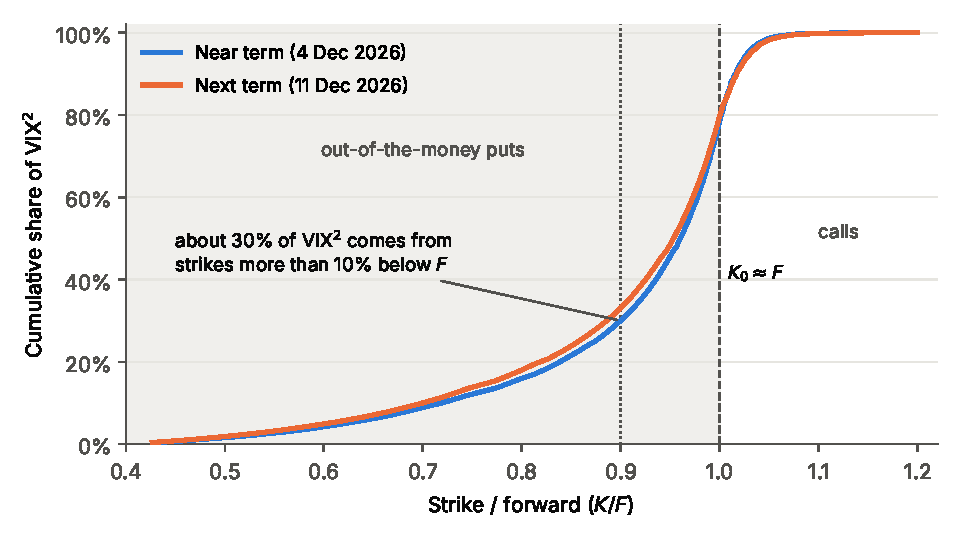
\includegraphics[width=0.85\linewidth]{figures/vix_strike_contributions.pdf}
  \caption{Cumulative share of $\sigma^2$ by strike, 5 November 2026 snapshot. About 76\% of the variance comes from out-of-the-money puts and 22\% from calls; roughly 30\% comes from puts more than 10\% below the forward.}
  \label{fig:contrib}
\end{figure}

Figure~\ref{fig:contrib} shows how the variance is built up across strikes. Puts supply about three quarters of VIX$^2$, and nearly a third comes from strikes more than 10\% below the forward. This is the combined effect of the $1/K^2$ weights and the skew: deep out-of-the-money puts are expensive because investors pay for crash protection. The VIX is therefore largely a price of crash insurance, which is why it rises sharply when the market falls.

\subsubsection{Numerical verification of the replication}

To confirm \eqref{eq:result} independently of Cboe's data, \texttt{verify\_variance\_replication.py} applies \eqref{eq:cboe} to option prices from two models in which the expected variance is known exactly. All prices use a forward of 100, $T=30/365$ and $r=4\%$.

\begin{table}[H]
\centering
\small
\begin{tabular}{@{}lrr@{}}
\toprule
\textbf{Strike grid} & \textbf{Strip variance} & \textbf{Volatility}\\
\midrule
Fine and wide (step 0.05, 20--300) & 0.040001 & 20.000\%\\
SPX-like spacing and range (step 0.07, 43--120) & 0.039997 & 19.999\%\\
Narrow range only (90--110) & 0.039056 & 19.763\%\\
Very coarse spacing only (step 5) & 0.045066 & 21.229\%\\
\bottomrule
\end{tabular}
\caption{Black--Scholes with $\sigma=20\%$ (true variance 0.04). The strip recovers the true variance; truncating the strike range lowers it and very coarse spacing raises it, as in Table~\ref{tab:assumptions}. A step of 0.07 at a forward of 100 matches SPX's 5-point spacing at 7,500.}
\label{tab:bs}
\end{table}

\begin{table}[H]
\centering
\small
\begin{tabular}{@{}lrr@{}}
\toprule
\textbf{Heston model, 200{,}000 Monte Carlo paths} & \textbf{Variance} & \textbf{Volatility}\\
\midrule
Exact expected variance $\theta+(v_0-\theta)\frac{1-e^{-\kappa T}}{\kappa T}$ & 0.028010 & 16.736\%\\
Simulated average realised variance & 0.028025 & 16.741\%\\
Option strip with $1/K^2$ weights & 0.028025 & 16.741\%\\
\bottomrule
\end{tabular}
\caption{Under Heston (parameters from \cite{gatheral}: $\kappa=1.3253$, $\theta=0.0354$, $\sigma=0.3877$, $\rho=-0.7165$; $v_0=0.0276=(16.61/100)^2$, the VIX close on 4 November 2026; full-truncation Euler, 24 steps per day), option prices are Monte Carlo averages over the same paths. The strip is within 0.1 standard errors of the exact value although volatility is random.}
\label{tab:heston}
\end{table}

Together, Tables~\ref{tab:cboe}--\ref{tab:heston} show that the formula is implemented correctly, that it reproduces the official index on live data, and that it recovers expected variance in a stochastic-volatility model, as the derivation predicts.


\subsection{Heston model: VIX futures, VIX calls and the convexity adjustment}
% Simulation: Heston model, VIX futures, VIX calls and the convexity adjustment (Daniel).
% Numbers and both tables come from heston/heston_vix.py; checks are in heston/test_heston_vix.py.

\subsubsection{Model and parameters}

Under the risk-neutral measure $\mathbb{Q}$ the Heston model lets the variance $v_t$ of the S\&P~500 move randomly while being pulled back toward a long run level:
\begin{equation}
  dS_t = rS_t\,dt + \sqrt{v_t}\,S_t\,dW^1_t, \qquad
  dv_t = \kappa(\theta - v_t)\,dt + \sigma\sqrt{v_t}\,dW^2_t, \qquad
  \operatorname{corr}(dW^1_t, dW^2_t) = \rho .
  \label{eq:heston}
\end{equation}
Here $S_t$ is the index level and $r$ is the risk-free rate. $W^1$ and $W^2$ are Brownian motions that drive the index and its variance, and their increments have correlation $\rho$. The parameter $\kappa$ is the speed at which $v_t$ returns to the long run variance $\theta$, and $\sigma$ is the volatility of variance. A negative $\rho$ makes volatility rise when the index falls.

The values of $\kappa$, $\theta$, $\sigma$ and $\rho$ come from Gatheral's textbook \cite{gatheral}, where Heston is fitted to S\&P~500 option prices. These describe how variance behaves in general. The starting variance $v_0$ describes one particular day, so we set it from the market's VIX on that day (Section~\ref{sec:hestonvix}). Table~\ref{tab:hestonparams} lists all five. Our prices depend only on $\kappa$, $\theta$, $\sigma$ and $v_0$. The correlation $\rho$ affects the index but not the VIX, which depends on $v_t$ alone (Section~\ref{sec:hestonvix}).

The Feller condition $2\kappa\theta \ge \sigma^2$ guarantees that $v_t$ stays strictly positive. Here $2\kappa\theta = 0.094 < \sigma^2 = 0.150$, so the condition fails and $v_t$ can reach zero. This is why the simulation uses full truncation (Section~\ref{sec:hestonsim}).

\begin{table}[H]
\centering
\small
\begin{tabular}{@{}llrl@{}}
\toprule
\textbf{Parameter} & \textbf{Meaning} & \textbf{Value} & \textbf{Source}\\
\midrule
$\kappa$ & speed of mean reversion (per year) & 1.3253 & Gatheral\\
$\theta$ & long run variance (VIX 18.8) & 0.0354 & Gatheral\\
$\sigma$ & volatility of variance & 0.3877 & Gatheral\\
$\rho$ & correlation of the two shocks & $-0.7165$ & Gatheral (does not affect VIX)\\
$v_0$ & variance on 3 November 2026 & 0.0438 & matched to VIX of 20.83\\
\bottomrule
\end{tabular}
\caption{Heston parameters. Gatheral's values are his fit to the S\&P~500 option surface of 15 September 2005 \cite[Table~3.2]{gatheral}\verify.}
\label{tab:hestonparams}
\end{table}

\subsubsection{The VIX under Heston}
\label{sec:hestonvix}

We first need the variance expected at a future date $s$, seen from today $t$. In the variance equation of \eqref{eq:heston} the random shocks average to zero, so on average each instant closes the same fraction $\kappa$ of the gap between $v$ and $\theta$. The gap is therefore discounted at rate $\kappa$, like a continuously compounded rate, which gives
\begin{equation}
  \EQ_t[v_s] = \theta + (v_t-\theta)\,e^{-\kappa(s-t)}, \qquad s \ge t.
  \label{eq:hestonmean}
\end{equation}
With $\kappa = 1.3253$ the gap halves about every six months.

$\VIX_t^2$ is the risk-neutral expected average variance over the next $\tau = 30/365$ years, so we average \eqref{eq:hestonmean} over that window. The long run part stays $\theta$. The gap part becomes today's gap times $B$, the average of the discount factor $e^{-\kappa u}$ over the 30 days, which is the average share of today's gap still present during the month. This gives an exact formula in $v_t$ alone:
\begin{equation}
  \VIX_t^2 = 100^2\,\EQ_t\!\left[\frac{1}{\tau}\int_t^{t+\tau} v_s\,ds\right]
  = 100^2\left[\theta + (v_t - \theta)\,B\right], \qquad B = \frac{1-e^{-\kappa\tau}}{\kappa\tau} = 0.9475 .
  \label{eq:hestonvix}
\end{equation}
VIX futures and options therefore depend only on $v$. We never simulate $S_t$, and $\rho$ plays no role.

We compare the model with the futures curve of 3 November 2026, the latest date in our futures data. The VIX closed at 20.83 that day. We can observe the VIX but not today's variance $v_0$, so we choose the $v_0$ that makes the model's VIX equal 20.83. Putting $\VIX = 20.83$ into \eqref{eq:hestonvix} and solving gives
\[
  v_0 = \theta + \frac{(20.83/100)^2 - \theta}{B} = 0.0438 .
\]

\subsubsection{Simulation}
\label{sec:hestonsim}

We simulate $v$ forward with an Euler scheme \cite{gatheral}, which replaces the continuous equation by daily steps of pull and random shock. We use $\Delta = 1/365$, 100{,}000 paths and random seed 42, out to 180 days. Because the Feller condition fails, a step can push $v$ below zero, so we use full truncation and replace $v$ by $v^+ = \max(v,0)$ in the pull and under the square root. One step is
\[
  v_{t+\Delta} = v_t + \kappa(\theta - v_t^+)\Delta + \sigma\sqrt{v_t^+\Delta}\;Z, \qquad Z\sim N(0,1),
\]
with a new $Z$ for every path and day. On each date $T$, every path's $v_T$ is converted into a $\VIX_T$ with \eqref{eq:hestonvix}. These simulated values of $\VIX_T$ are used to price the futures and calls below. The Monte Carlo standard error, the typical change in a price if we reran with new random numbers, is at most 0.03 VIX points for futures and 0.02 points for calls.

To test the simulation we compared it with results known in advance. On day 0 the model's VIX is exactly 20.83, the market close on 3 November. The average variance also has an exact formula \eqref{eq:hestonmean}. Table~\ref{tab:hestonchecks} compares it with the simulated average on days 30 and 91, the call maturities, and on day 180, the last simulated day. Every difference is smaller than the random error. Finally, rerunning with 200{,}000 paths changes no price by more than 0.012 points for futures and 0.010 points for calls\unskip.

\begin{table}[H]
\centering
\small
\begin{tabular}{@{}lrrrr@{}}
\toprule
\textbf{Day} & \textbf{Simulated $\EQ[v_T]$} & \textbf{Exact $\EQ[v_T]$} & \textbf{Difference} & \textbf{Random error (2 s.e.)}\\
\midrule
30 & 0.04306 & 0.04296 & +0.24\% & 0.33\% \\
91 & 0.04150 & 0.04146 & +0.10\% & 0.52\% \\
180 & 0.03966 & 0.03979 & -0.31\% & 0.66\% \\
\bottomrule
\end{tabular}

\caption{Simulated against exact average variance. The random error is two standard errors, the range within which about 95\% of reruns would fall.}
\label{tab:hestonchecks}
\end{table}

\subsubsection{Futures curve vs market}

A VIX future pays $\VIX_T$ and costs nothing to enter, so its price is $F(T) = \EQ[\VIX_T]$, the average of $\VIX_T$ over the paths. Figure~\ref{fig:hestoncurve} and Table~\ref{tab:hestonfutures} compare it with the settlements of 3 November 2026.

\begin{figure}[H]
\centering
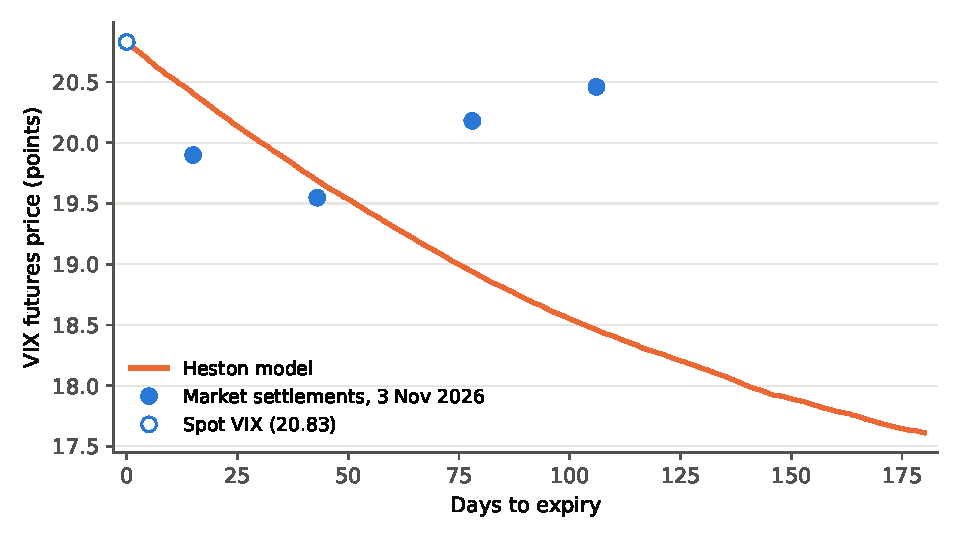
\includegraphics[width=0.85\linewidth]{figures/heston_futures_curve.pdf}
\caption{VIX futures curve on 3 November 2026. Market settlements and the Heston model started at the spot VIX.}
\label{fig:hestoncurve}
\end{figure}

\begin{table}[H]
\centering
\small
\begin{tabular}{@{}lrrrr@{}}
\toprule
\textbf{Expiry} & \textbf{Days} & \textbf{Market} & \textbf{Model} & \textbf{Market $-$ model}\\
\midrule
2026-11-18 & 15 & 19.90 & 20.41 & -0.51 \\
2026-12-16 & 43 & 19.55 & 19.69 & -0.14 \\
2027-01-20 & 78 & 20.18 & 18.94 & +1.24 \\
2027-02-17 & 106 & 20.46 & 18.46 & +2.00 \\
2027-03-17 & 134 & 20.58 & 18.09 & +2.49 \\
2027-04-21 & 169 & 20.93 & 17.70 & +3.22 \\
\bottomrule
\end{tabular}

\caption{VIX futures on 3 November 2026, in VIX points ($\$1{,}000$ per point). Days are calendar days to expiry.}
\label{tab:hestonfutures}
\end{table}

Because $v_0 > \theta$, the model curve falls from 20.83 toward the long run level and reaches 17.6 after 180 days. The market curve is roughly flat, dipping to 19.55 and rising to 20.93. The model is 0.5 points too high at the front and 3.2 points too low at the April contract. There are two reasons. The parameters were fitted to S\&P~500 options, not to VIX futures. And a model with a single variance factor can only move in one direction from today's VIX toward $\theta$, so it cannot produce a curve that dips and then rises. This is a known limitation of such models for VIX futures \cite{bergomi,gatheral2008}.

\subsubsection{VIX call prices}

A VIX call pays $\max(\VIX_T - K, 0)$ at expiry, so its price $C(K,T) = e^{-rT}\,\EQ[\max(\VIX_T - K,0)]$ is the discounted average payoff over the same paths. We discount with the 1 month (30 days) and 3 month (91 days) Treasury yields of 3 November 2026, converted to continuous compounding as in the VIX calculation above. Table~\ref{tab:hestoncalls} lists the prices. One option contract is worth $\$100$ per VIX point.

\begin{table}[H]
\centering
\small
\begin{tabular}{@{}lrrrr@{}}
\toprule
& \multicolumn{2}{c}{\textbf{1 month (30 days)}} & \multicolumn{2}{c}{\textbf{3 months (91 days)}}\\
\cmidrule(lr){2-3}\cmidrule(lr){4-5}
\textbf{Strike} & \textbf{Points} & \textbf{Per contract} & \textbf{Points} & \textbf{Per contract}\\
\midrule
15 & 5.43 & \$543 & 5.26 & \$526 \\
20 & 2.05 & \$205 & 2.59 & \$259 \\
25 & 0.46 & \$46 & 1.03 & \$103 \\
30 & 0.05 & \$5 & 0.33 & \$33 \\
\bottomrule
\end{tabular}

\caption{Heston VIX call prices on 3 November 2026, in VIX points and dollars per contract ($\$100$ per point).}
\label{tab:hestoncalls}
\end{table}

Prices fall as the strike rises. Calls with strikes 20, 25 and 30 are worth more at 3 months, because $\VIX_T$ is more uncertain further out. The call with strike 15 is already well in the money and is worth slightly less at 3 months, because the model's futures price falls from 20.0 to 18.7 between the two dates.
\subsubsection{Convexity adjustment}
\label{sec:hestonconv}

The variance swap replication \eqref{eq:result} shows that option prices fix the price of $\VIX^2$, the variance. A VIX future, however, pays $\VIX$ itself, the square root. If $\VIX_T$ were known for certain, $\sqrt{\EQ[\VIX_T^2]}$ and $\EQ[\VIX_T]$ would be equal. Because $\VIX_T$ is uncertain and the square root is concave, Jensen's inequality makes the first larger. We call the gap the convexity adjustment (CA):
\[
  \mathrm{CA}(T) = \sqrt{\EQ[\VIX_T^2]} - \EQ[\VIX_T] \;\ge\; 0 .
\]
For each date $T$ from 1 to 180 days we compute both terms. $\EQ[\VIX_T^2]$ follows exactly from \eqref{eq:hestonmean} and \eqref{eq:hestonvix}, since $\VIX_T^2$ is linear in $v_T$, and $\EQ[\VIX_T]$ is the simulated futures price. Figure~\ref{fig:hestonconvexity} shows the difference, which is 0.62 points at 30 days, 1.58 at 91 days and 2.28 at 180 days. It grows with maturity because the range of possible values of $\VIX_T$ widens the further ahead we look. This is why a VIX future cannot be priced as the square root of a variance swap.

\begin{figure}[H]
\centering
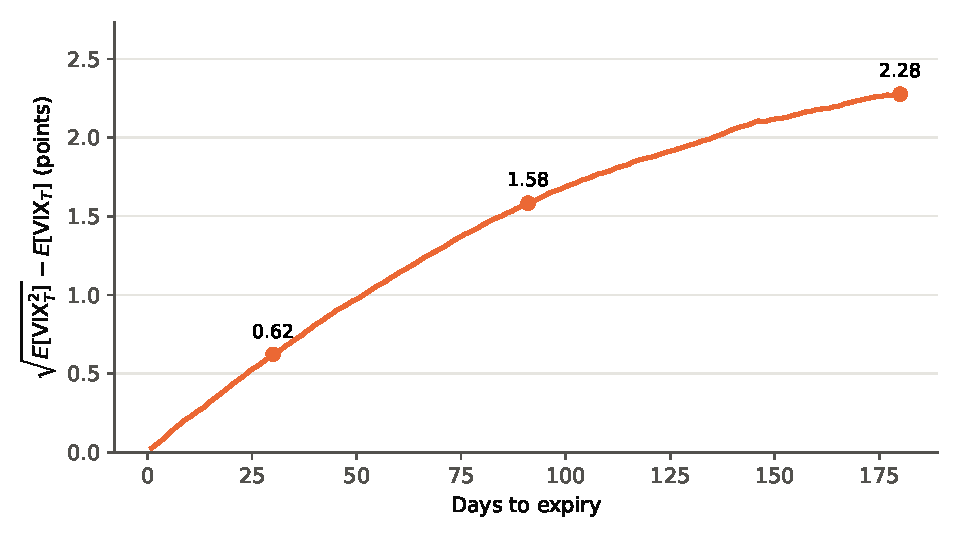
\includegraphics[width=0.85\linewidth]{figures/heston_convexity.pdf}
\caption{Convexity adjustment $\sqrt{\EQ[\VIX_T^2]} - \EQ[\VIX_T]$ under Heston, started at the spot VIX of 3 November 2026.}
\label{fig:hestonconvexity}
\end{figure}

\subsubsection{Limitations}

Heston has a single variance factor, so it ties the whole futures curve to today's VIX and cannot fit a curve that dips and then rises. That would need a second variance factor. Gatheral's parameters were fitted to S\&P~500 options, not to VIX futures or options, and here we adjusted only $v_0$. Daily Euler steps add discretisation error, but the checks against the exact means show it is smaller than the Monte Carlo error.


\subsection{Hedging backtest}
% Hedging backtest figures (Tony).
% Generated by hedging_backtest.py and report/make_hedging_figures.py.

The backtest overlays a long front-month VIX-futures position on a \$1M SPY
portfolio. The hedge ratio is re-estimated each month from the previous 252
trading days (with a 504-day window as a robustness check), using only
information available at the rebalance date. Figures~\ref{fig:hedge-ratio}
to~\ref{fig:hedging-crises} show the resulting hedge-size path, the portfolio
and drawdown paths, the roll-cost decomposition, and the returns in the 2018
and 2020 stress episodes.

\begin{figure}[H]
  \centering
  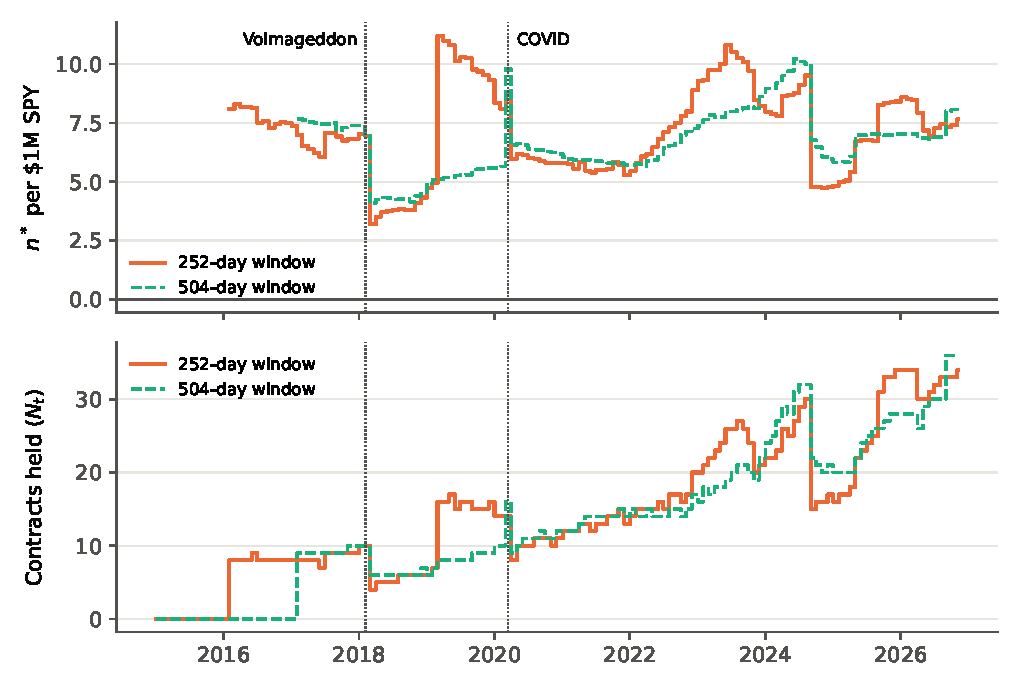
\includegraphics[width=0.95\linewidth]{figures/hedge_ratio_rolling.pdf}
  \caption{Rolling variance-minimizing hedge size. Top: $n^*$ per \$1M of SPY.
  Bottom: actual number of VX contracts held. The first 252 (504) trading days
  are an estimation warm-up with no hedge. Dotted lines mark 5 February 2018
  and 16 March 2020.}
  \label{fig:hedge-ratio}
\end{figure}

\begin{figure}[H]
  \centering
  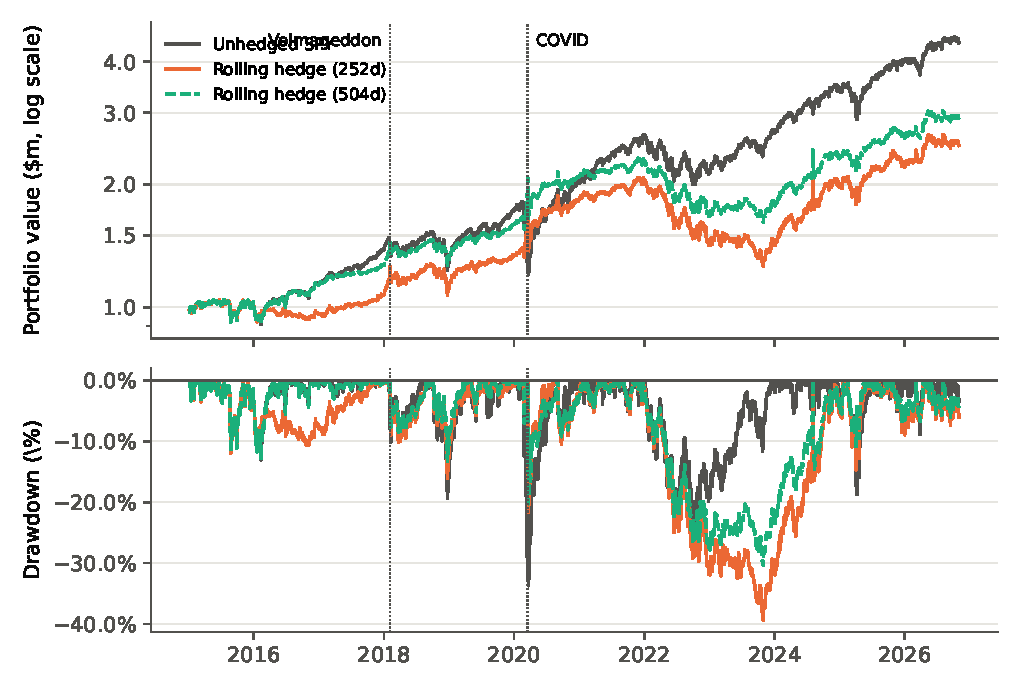
\includegraphics[width=0.95\linewidth]{figures/hedging_equity.pdf}
  \caption{Hedged and unhedged \$1M SPY portfolios. Top: portfolio value on a
  log scale. Bottom: drawdown. The rolling hedge reduces volatility and protects
  in crises, but the 252-day version suffers a prolonged roll-cost drawdown in
  2022--2023.}
  \label{fig:hedging-equity}
\end{figure}

\begin{figure}[H]
  \centering
  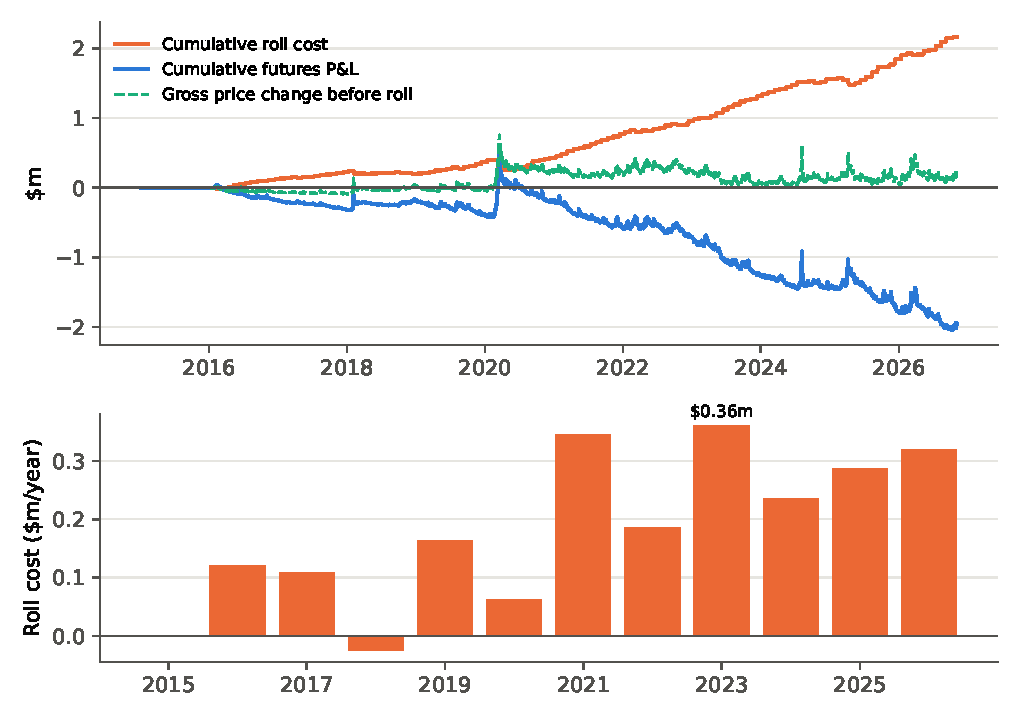
\includegraphics[width=0.95\linewidth]{figures/hedging_roll_cost.pdf}
  \caption{Cumulative roll cost and futures P\&L for the 252-day rolling hedge.
  The roll cost is the dominant drag: gross price change before roll is small.
  Bottom: annual roll cost.}
  \label{fig:hedging-roll-cost}
\end{figure}

\begin{figure}[H]
  \centering
  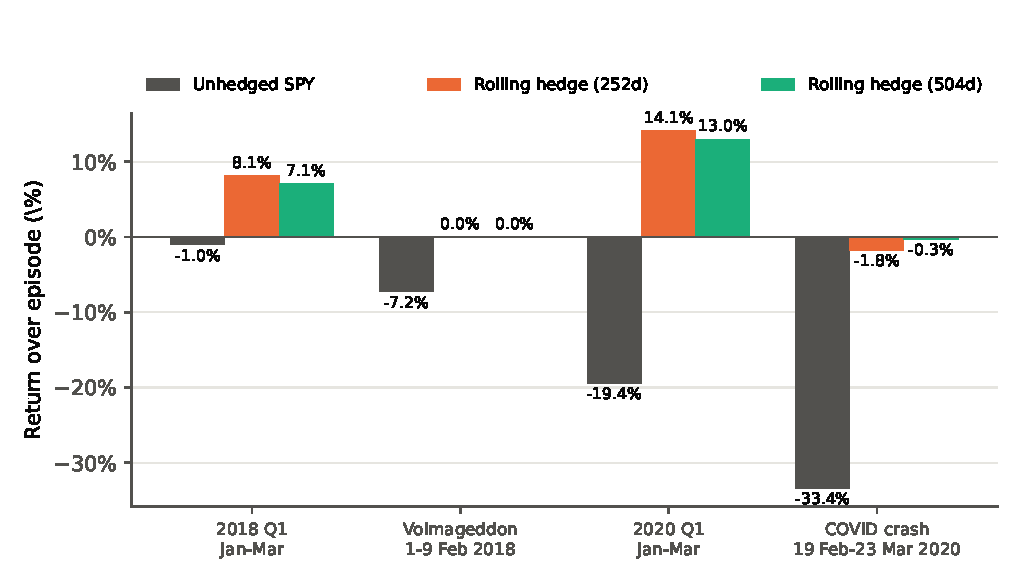
\includegraphics[width=0.95\linewidth]{figures/hedging_crises.pdf}
  \caption{Returns over crisis episodes. The rolling hedge turns the 2020 Q1
  loss into a gain and nearly neutralizes the COVID crash, but over-hedges in
  the calm run-up to 2018.}
  \label{fig:hedging-crises}
\end{figure}


%=====================================================================
\section{Conclusion}
%=====================================================================
\paragraph{The index and its products.} The VIX measures the market's expected S\&P~500 volatility over the next 30 days, read from option prices rather than past returns. It rises sharply when equities fall, which makes it the market's ``fear gauge'' and a natural hedge. Because the index itself cannot be traded, exposure comes through futures, options and exchange-traded products. These products track futures, not spot, so long-volatility ETPs such as VXX lose value steadily in contango, and the daily-reset inverse products that profited from that decay were wiped out in a single day in February 2018.

\paragraph{Pricing.} Using It\^o's lemma and the Carr--Madan replication of the log contract, we showed that $\VIX^2$ is the fair strike of a 30-day variance swap and that it can be read from a strip of out-of-the-money options weighted by $1/K^2$, with no volatility model. The Cboe formula is the discrete version of this result. Our implementation reproduces every intermediate value of Cboe's worked example and computes a live VIX of 22.49 against the official 22.54, and the replication recovers the true expected variance under both Black--Scholes and Heston. On the live data about three quarters of $\VIX^2$ comes from out-of-the-money puts, so the VIX is largely a price of crash insurance.

\paragraph{Futures versus spot.} A VIX future is the risk-neutral expectation of the VIX at expiry, not today's VIX, and because the square root is concave it lies below the square root of forward variance. Under Heston this convexity adjustment is 0.62 points at 30 days, 1.58 at 91 days and 2.28 at 180 days. With parameters fitted to S\&P~500 options, the model is 0.5 points too high at the front of the 3~November~2026 curve and 3.2 points too low at 169 days: a single variance factor can only move monotonically from today's VIX toward its long-run level.

\paragraph{Hedging.} Equity returns and VIX futures are strongly negatively correlated, so a long VIX-futures position reduces portfolio risk. In our 2015--2026 backtest the rolling variance-minimising hedge reduced the variance of daily returns by 14\% (252-day estimation window) and 31\% (504-day window), turned a 19\% loss in the first quarter of 2020 into a 13--14\% gain, and limited the COVID-crash loss to under 2\% against 33\% unhedged. The price is the roll cost: futures in contango converge down to spot, which cost about \$180{,}000 a year, or 12\% of the average portfolio value, and cut the annual return from 13.5\% to 8.0\% (252-day window) and 9.4\% (504-day window). With the shorter window the hedge also deepened the 2022--2023 drawdown. VIX futures are therefore effective crisis insurance but an expensive permanent hedge.

\paragraph{Limitations.} Our option quotes are 15-minute delayed Yahoo Finance data, and our rate curve uses two points rather than Cboe's spline. The Heston parameters were not calibrated to VIX futures or options, and only the starting variance was fitted. The backtest uses daily settlement prices and ignores commissions and bid--ask spreads, which would add to the cost of rolling.

%=====================================================================
\appendix
% Appendix: data and code (Nikita).

\section{Data and code}
\begin{table}[H]
\centering
\small
\footnotesize
\begin{tabular}{@{}p{6.0cm}p{4.8cm}p{2.8cm}@{}}
\toprule
\textbf{File} & \textbf{Contents} & \textbf{Source}\\
\midrule
\texttt{data/options/}\newline\texttt{spx\_options\_20261105\_1141.csv} & SPX/SPXW options 20--40 days out, with spot and official VIX & Yahoo Finance\\
\texttt{data/risk\_free.csv} & Daily 1- and 3-month Treasury yields, 2010--2026 & US Treasury\\
\texttt{data/market\_history.csv} & Daily VIX, S\&P~500 and SPY (dividend-adjusted), 2010--2026 & Yahoo Finance\\
\texttt{data/vix\_futures\_all.csv} & Daily settlements of every monthly VX contract, Jan 2015--Feb 2027 & Cboe Futures Exchange\\
\texttt{data/vix\_front\_month.csv} & Front-month series rolled 5 trading days before expiry (used in the backtest) & Built from the above\\
\texttt{references/}\newline\texttt{cboe\_example\_*.csv} & Option data of Cboe's worked example & Cboe White Paper, App.~1\\
\midrule
\texttt{vix\_calc.py} & Computes the VIX from a snapshot & \\
\texttt{check\_cboe\_example.py} & Reproduces Table~\ref{tab:cboe} & \\
\texttt{verify\_variance\_replication.py} & Reproduces Tables~\ref{tab:bs}--\ref{tab:heston} & \\
\texttt{report/make\_vix\_figures.py} & Draws Figure~\ref{fig:contrib} & \\
\bottomrule
\end{tabular}
\end{table}


%=====================================================================
\begin{thebibliography}{99}
\bibitem{cboewp} Cboe (2019). \emph{Cboe Volatility Index White Paper}. \url{https://www.asx.com.au/content/dam/asx/investors/investment-options/vix/cboe-vix-white-paper.pdf}
\bibitem{cboemeth} Cboe Global Indices. \emph{Cboe Volatility Index Mathematics Methodology}.
\bibitem{carrmadan} P.~Carr and D.~Madan (1998). Towards a theory of volatility trading. In R.~Jarrow (ed.), \emph{Volatility: New Estimation Techniques for Pricing Derivatives}, Risk Books.
\bibitem{ddkz} K.~Demeterfi, E.~Derman, M.~Kamal and J.~Zou (1999). \emph{More than you ever wanted to know about volatility swaps}. Goldman Sachs Quantitative Strategies Research Notes.
\bibitem{carrwu} P.~Carr and L.~Wu (2009). Variance risk premiums. \emph{Review of Financial Studies}, 22(3).
\bibitem{whaley} R.~E.~Whaley (2009). Understanding the VIX. \emph{Journal of Portfolio Management}, 35(3), 98--105.
\bibitem{vxx} Barclays Bank PLC (2018). iPath Series~B S\&P~500 VIX Short-Term Futures ETN, pricing supplement (Form 424B2), 17 January 2018. SEC EDGAR.
\bibitem{augustin} P.~Augustin, I.-H.~Cheng and L.~Van den Bergen (2021). Volmageddon and the failure of short volatility products. \emph{Financial Analysts Journal}, 77(3), 35--51.
\bibitem{csxiv} Credit Suisse AG (2018). Credit Suisse AG announces event acceleration of its XIV ETNs. Press release, 6 February 2018.
\bibitem{bbgvol} Bloomberg News (2018). Tiny vol products helped fuel market's slump. Reprinted in \emph{InvestmentNews}, 7 February 2018.
\bibitem{proshares} ProShares. Short VIX Short-Term Futures ETF (SVXY), fund page: daily objective changed from $-1\times$ to $-0.5\times$ at the close of 27 February 2018. \url{https://www.proshares.com/funds/svxy_performance_and_quote.html}
\bibitem{hull} J.~C.~Hull (2022). \emph{Options, Futures, and Other Derivatives}, 11th ed. Pearson.
\bibitem{shreve} S.~E.~Shreve (2004). \emph{Stochastic Calculus for Finance II: Continuous-Time Models}. Springer.
\bibitem{gatheral} J.~Gatheral (2006). \emph{The Volatility Surface: A Practitioner's Guide}. Wiley.
\bibitem{bergomi} L.~Bergomi (2005). Smile dynamics II. \emph{Risk}, 18(10), 67--73.
\bibitem{gatheral2008} J.~Gatheral (2008). Consistent modeling of SPX and VIX options. Presentation, Fifth World Congress of the Bachelier Finance Society, London, 18 July 2008.
\end{thebibliography}

\end{document}
